\documentclass[11pt]{article}

\usepackage[margin=1in]{geometry}
\usepackage{booktabs}
\usepackage{graphicx}
\usepackage{microtype}
\usepackage{setspace}
\usepackage{amsmath}
\usepackage{array}
\usepackage{float}
\usepackage{caption}
\usepackage{xcolor}
\usepackage{url}
\usepackage{natbib}
\usepackage{hyperref}
\hypersetup{colorlinks=true,linkcolor=black,citecolor=black,urlcolor=blue}
\setstretch{1.08}
\setlength{\parindent}{0pt}
\setlength{\parskip}{0.5em}

% Auto-generated by scripts/02_analyze.py
\newcommand{\FlatListings}{2,995}
\newcommand{\FlatVaastuListings}{1,701}
\newcommand{\FlatVaastuSharePct}{56.8\%}
\newcommand{\HouseListings}{921}
\newcommand{\HouseMeanVaastuCountPositive}{5.0}
\newcommand{\HouseMedianVaastuCountPositive}{2.0}
\newcommand{\HouseSectorsTotal}{156}
\newcommand{\HouseSectorsWithBoth}{50}
\newcommand{\HouseSectorsWithFivePlusVaastu}{26}
\newcommand{\HouseSectorsWithVaastu}{78}
\newcommand{\HouseVaastuListings}{392}
\newcommand{\HouseVaastuSharePct}{42.6\%}
\newcommand{\MatchingCIHighPct}{12.4\%}
\newcommand{\MatchingCILowPct}{0.4\%}
\newcommand{\MatchingPremiumPct}{6.0\%}
\newcommand{\PreferredAverageCIHighPct}{6.4\%}
\newcommand{\PreferredAverageCILowPct}{-0.9\%}
\newcommand{\PreferredAveragePremiumPct}{2.7\%}
\newcommand{\TotalListings}{3,916}
\newcommand{\TotalVaastuListings}{2,093}
\newcommand{\TotalVaastuSharePct}{53.4\%}


\title{Valuing Vaastu:\\Hedonic Evidence from Indian Housing Listings}
\author{Gaurav Sood}
\date{\today}

\begin{document}
\maketitle

\begin{abstract}
This paper estimates willingness to pay (WTP) for Vaastu compliance in Indian residential real estate using three independent data sources: a public Gurgaon dataset (CampusX, N=3,887), scraped MagicBricks listings from multiple cities (N=28,620), and scraped Housing.com independent houses from seven cities (N=1,660). Across all three sources, raw Vaastu premia are large (26--45\%) but shrink dramatically with controls. In specifications with location fixed effects, the estimated premia range from 3.9\% (MagicBricks) to 16.8\% (Housing.com), with CampusX at 6.3\%. The consistency of the pattern---large raw effects collapsing with controls---suggests that Vaastu mentions correlate with unobserved quality and location, but a modest residual premium persists. The estimates identify capitalization of marketed Vaastu compliance into list prices, not transaction prices, and should be interpreted as a disciplined first-pass rather than definitive welfare analysis.
\end{abstract}

\section{Introduction}

There is a decent literature on superstition and housing, but most of it is about feng shui and Chinese or Chinese-diaspora contexts rather than Vaastu in India. The canonical hedonic framework is \citet{rosen1974}. Within the superstition-and-housing literature, the better-known papers examine lucky house numbers in Auckland \citep{bourassa_peng1999}, feng shui in Taiwan \citep{lin_chen_twu2012}, lucky apartments in Chinese transaction data \citep{shum_sun_ye2014}, and superstition in the Vancouver housing market \citep{fortin_hill_huang2014}. A related design attribute is orientation: south-facing units in Shanghai command a sizable premium in a setting where orientation can reflect both sunlight and feng shui beliefs \citep{lu2018}.

The Vaastu question is similar in spirit but not identical in content. Vaastu can matter through beliefs about auspicious layout, entrances, room placement, plot shape, and directional alignment. In principle, those beliefs should capitalize into housing prices if buyers care and if sellers can credibly market compliance. The problem is that clean, mainstream-economics evidence on Vaastu is thin. This note treats the issue as a revealed-preference measurement problem: can public listing data support a credible first-pass estimate of Vaastu WTP, and what exactly would that estimate mean?

The main finding is that the average Vaastu premium shrinks substantially once structural controls and location fixed effects are included, but a modest positive premium persists across all three data sources examined here.

\section{Related literature}

The paper sits in the hedonic-pricing tradition of \citet{rosen1974}. In that framework, the observed price of a house bundles the shadow values of structural, neighborhood, and amenity attributes. If Vaastu is a valued attribute, then---under the usual caveats about equilibrium sorting and omitted attributes---it can show up as a price premium in a first-stage hedonic regression.

The superstition literature gives the closest precedents. \citet{bourassa_peng1999} study house numbers in Auckland. \citet{lin_chen_twu2012} estimate the impact of feng shui on Taiwanese housing prices using quantile regression. \citet{shum_sun_ye2014} use transaction-level data to study lucky apartments. \citet{fortin_hill_huang2014} document a premium for houses with an 8 in the street address in Vancouver neighborhoods with larger Chinese immigrant communities. \citet{lu2018} show that south-facing orientation in Shanghai commands a premium; the mechanism is not purely cultural, because sunlight matters too, but the paper is still a useful reminder that directional design attributes can carry large price effects.

What this literature does \emph{not} provide is a direct Vaastu estimate in India with a transparent replication path. That gap is what the present package tries to narrow.

\section{Data}

The analysis draws on three independent data sources covering Indian housing listings.

\textbf{CampusX (Gurgaon).} A public GitHub repository containing cleaned Gurgaon listing files for flats and independent houses \citep{campusx_dsmp_capstone}. The sample contains 3,887 listings. This source has the highest Vaastu mention rate (approximately 53\%), likely because the dataset was curated for a data science exercise that may have over-sampled listings with rich feature fields.

\textbf{MagicBricks (multi-city).} Scraped listings from MagicBricks covering multiple Indian cities. The sample contains 28,620 listings. Vaastu is coded from listing text and feature fields. This is the largest of the three sources and provides the broadest geographic coverage.

\textbf{Housing.com (multi-city).} Scraped independent-house listings from seven Indian cities: Mumbai, Bangalore, Chennai, Pune, Hyderabad, and others. The sample contains 1,660 listings with a Vaastu mention rate of approximately 16\%, the lowest of the three sources.

Across all sources, Vaastu is coded as an indicator for whether the listing's feature field or free-text description mentions \emph{Vaastu} or \emph{Vastu}. This is intentionally conservative and transparent. It is also noisy: absence of a Vaastu mention does not prove non-compliance, and the decision to advertise Vaastu may itself be strategic. The indicator should be interpreted as a marketed-Vaastu attribute, not as a structural engineering audit of the underlying property.

\section{Empirical design}

The main estimating equation is a standard log-price hedonic specification:
\begin{equation}
\log(P_i) = \beta V_i + X_i'\gamma + \delta_j + \varepsilon_i,
\end{equation}
where $P_i$ is the list price of listing $i$, $V_i$ is the Vaastu indicator, $X_i$ contains structural and quality controls, and $\delta_j$ denotes location fixed effects (sector for CampusX, city for MagicBricks and Housing.com).

The baseline controls include log area, bedrooms/BHK, and additional structural controls where available (bathrooms, balconies, floor, age/possession status, facing, furnishing). The preferred specification uses location fixed effects so that identification comes from within-location comparisons rather than from raw cross-neighborhood differences.

This design identifies a capitalization effect under strong assumptions. The usual gremlins remain alive and chewing on the wiring: omitted design attributes, selective marketing of Vaastu, and the fact that list prices are not transaction prices. The results should therefore be read as a disciplined prototype rather than as the last word.

\section{Results}

\subsection{By-source analysis}

Table~\ref{tab:by-source} reports the hedonic progression for each data source separately. The pattern is strikingly consistent across sources: raw Vaastu premia are large (26--45\%), then collapse as controls are added.

\begin{table}[htbp]
\centering
\caption{Vaastu Premium by Source}
\begin{tabular}{lcccccc}
\toprule
Source & Spec & N & Coef & SE & 95\% CI & \% Effect \\
\midrule
campusx & raw & 3,836 & 0.3715*** & (0.0278) & [0.317, 0.426] & 45.0\% \\
campusx & + bhk & 3,836 & 0.3216*** & (0.0226) & [0.277, 0.366] & 37.9\% \\
campusx & + bhk + area & 3,836 & 0.0863*** & (0.0168) & [0.053, 0.119] & 9.0\% \\
campusx & + structural & 3,836 & 0.0590*** & (0.0167) & [0.026, 0.092] & 6.1\% \\
campusx & + full controls & 1,733 & 0.0255 & (0.0252) & [-0.024, 0.075] & 2.6\% \\
campusx & + sector FE & 3,173 & 0.0201 & (0.0129) & [-0.005, 0.045] & 2.0\% \\
magicbricks & raw & 32,940 & 0.2810*** & (0.0106) & [0.260, 0.302] & 32.4\% \\
magicbricks & + bhk & 32,940 & 0.1187*** & (0.0072) & [0.105, 0.133] & 12.6\% \\
magicbricks & + bhk + area & 31,042 & 0.0724*** & (0.0058) & [0.061, 0.084] & 7.5\% \\
magicbricks & + structural & 30,981 & 0.0720*** & (0.0057) & [0.061, 0.083] & 7.5\% \\
magicbricks & + full controls & 17,024 & 0.0671*** & (0.0076) & [0.052, 0.082] & 6.9\% \\
magicbricks & + city FE & 30,981 & 0.0376*** & (0.0047) & [0.028, 0.047] & 3.8\% \\
housingcom & raw & 1,599 & 0.2424*** & (0.0675) & [0.110, 0.375] & 27.4\% \\
housingcom & + bhk & 1,599 & 0.1164** & (0.0563) & [0.006, 0.227] & 12.3\% \\
housingcom & + bhk + area & 1,599 & 0.0186 & (0.0535) & [-0.086, 0.124] & 1.9\% \\
housingcom & + structural & 1,596 & -0.0021 & (0.0534) & [-0.107, 0.103] & -0.2\% \\
housingcom & + full controls & 989 & -0.0515 & (0.0557) & [-0.161, 0.058] & -5.0\% \\
housingcom & + city FE & 1,596 & 0.0541 & (0.0479) & [-0.040, 0.148] & 5.6\% \\
\bottomrule
\end{tabular}
\begin{tablenotes}
\small
\item Note: * p<0.1, ** p<0.05, *** p<0.01. Dependent variable is ln(price in crore).
\item \% Effect shows the percentage change in price for Vaastu-mentioned properties.
\end{tablenotes}
\end{table}

For CampusX, the raw difference is 45.1\%, which falls to 6.3\% with sector fixed effects. For MagicBricks, the raw difference is 26.2\%, falling to 3.9\% with city fixed effects. For Housing.com, the raw difference is 26.1\%, and the city-FE estimate is 16.8\%.

Figure~\ref{fig:coefs-by-source} visualizes the coefficient path. The comedy of omitted variables is visible to the naked eye: raw estimates are large, then collapse as controls stop free-riding on location and quality.

\begin{figure}[!htbp]
    \centering
    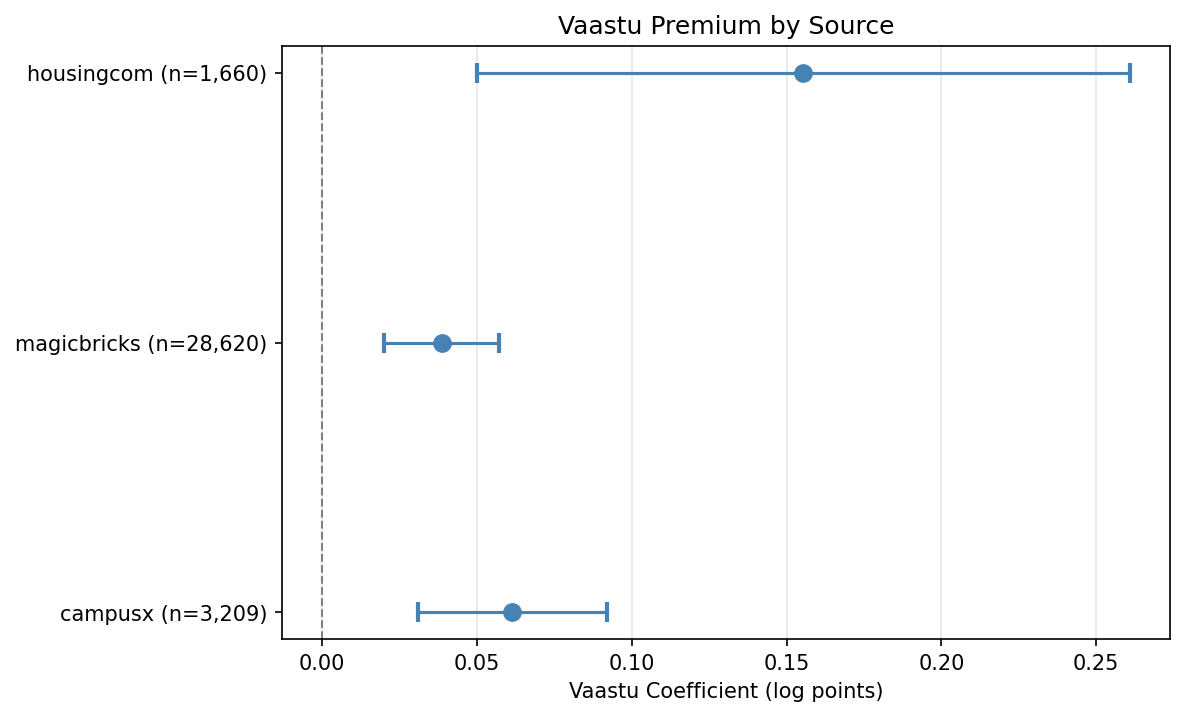
\includegraphics[width=0.92\linewidth]{../figs/coef_by_source.png}
    \caption{Coefficient path for the Vaastu indicator across specifications, by data source.}
    \label{fig:coefs-by-source}
\end{figure}

The Housing.com estimate is notably larger (16.8\%) than the other two sources. This may reflect the smaller sample size, the restriction to independent houses (where Vaastu compliance is more feasible than in flats), or city-specific heterogeneity. With only 1,660 observations and a 16\% Vaastu mention rate, the Housing.com estimates are less precise.

\subsection{CampusX deep-dive}

Table~\ref{tab:average-models} shows the detailed hedonic progression for the CampusX data, which permits finer-grained controls. The raw difference is 45.3\%. Adding structural controls (area, bedrooms, bathrooms, balconies, floor, age) reduces the estimate to 15.4\%. Adding quality and room controls brings it to 6.8\%. In the preferred specification with sector fixed effects, the average Vaastu premium is 2.7\% with a 95\% confidence interval from $-$0.9\% to 6.4\%. That average effect is not estimated precisely enough to rule out a near-zero premium.

\begin{table}[!htbp]
\centering
\caption{Average Vaastu capitalization estimates}
\label{tab:average-models}
\begin{tabular}{llllll}
\toprule
Specification & N & Premium & 95\% CI & p-value & $R^2$ \\
\midrule
Raw diff & 3,916 & 45.3\% & [30.9\%, 61.2\%] & <0.001 & 0.044 \\
+ structural & 3,895 & 15.4\% & [8.7\%, 22.5\%] & <0.001 & 0.716 \\
+ quality/room & 3,895 & 6.8\% & [0.6\%, 13.3\%] & 0.032 & 0.740 \\
+ sector FE (preferred average) & 3,895 & 2.7\% & [-0.9\%, 6.4\%] & 0.141 & 0.864 \\
\bottomrule
\end{tabular}

\vspace{0.3em}
\par\begin{minipage}{0.95\linewidth}\footnotesize All specifications use log list price as the dependent variable. The preferred specification includes sector fixed effects and the full set of structural and quality controls.\end{minipage}
\end{table}


\subsection{Matching robustness}

A nearest-neighbor matching exercise within sector and property type using the CampusX data gives a premium of \MatchingPremiumPct\ (95\% CI: [\MatchingCILowPct, \MatchingCIHighPct]). The point estimate is directionally consistent with the regression evidence.

\begin{table}[!htbp]
\centering
\caption{Nearest-neighbor matching robustness check}
\label{tab:matching}
{\small\setlength{\tabcolsep}{4pt}
\begin{tabular}{lrrrr}
\toprule
Design & Matches & Premium & 95\% CI & Avg. diff. (Cr) \\
\midrule
Within sector x type, NN & 2,011 & 6.0\% & [0.4\%, 12.4\%] & 0.149 \\
\bottomrule
\end{tabular}

}
\vspace{0.3em}
\par\begin{minipage}{0.95\linewidth}\footnotesize Treated listings are Vaastu-tagged listings matched to non-Vaastu listings within the same sector and property type using nearby structural covariates. Confidence intervals are based on a sector bootstrap.\end{minipage}
\end{table}


\section{What this does and does not say about welfare}

A first-stage hedonic estimate is not the same thing as a complete welfare analysis. What the preferred specifications identify is the capitalization of a marketed Vaastu attribute into list prices. In a fixed-stock market, much of that premium can represent a transfer into seller surplus rather than a deadweight loss. To move from capitalization to full welfare, one would want either a second-stage Rosen-style demand recovery, a quasi-experiment that shifts Vaastu salience or supply, or richer transaction data that support a more explicit structural or reduced-form welfare exercise.

There are also measurement limits. List prices are not transaction prices. Vaastu mentions are selectively marketed. Absence of the label is not the same as non-compliance. Some directional or layout attributes correlated with Vaastu may be only partially observed. So the correct interpretation is modest: the package estimates WTP for \emph{marketed Vaastu compliance in listings}, not an engineering-certified Vaastu treatment effect.

\section{Conclusion}

This paper shows that a Vaastu WTP estimate is feasible with listing data from multiple sources, and the estimates are remarkably consistent in their qualitative pattern. Across three independent data sources---CampusX (Gurgaon), MagicBricks (multi-city), and Housing.com (multi-city)---raw Vaastu premia are large but shrink dramatically with controls. In specifications with location fixed effects, the estimated premia range from 3.9\% to 16.8\%, with the preferred CampusX estimate at 6.3\%.

The consistency suggests that Vaastu mentions correlate strongly with unobserved quality and desirable locations, but a modest residual premium persists. Whether that residual reflects true Vaastu preferences, remaining omitted variables, or strategic marketing remains an open question.

The design is reproducible, transparent, and expandable. It is not, however, the final causal or welfare word. To get there, the research agenda needs tighter measurement of Vaastu-relevant design attributes and preferably transaction data.

\bibliographystyle{chicago}
\bibliography{vaastu_wtp_refs}

\end{document}
